\chapter{JPEG}

\section{Overview}

JPEG, which stands for Joint Photographic Experts Group (the name of the committee that created the JPEG standard) is a lossy compression algorithm for images. A lossy compression scheme is a way to inexactly represent the data in the image, such that less memory is used yet the data appears to be very similar. This is why JPEG images look almost the same as the original images they were derived from most of the time unless the quality is reduced significantly, in which case there will be visible differences.

The JPEG algorithm takes advantage of the fact that humans can't see colors at high frequencies. These high frequencies are the data points in the image that are eliminated during the compression. JPEG compression also works best on images with smooth colour transitions.

JPEG is a commonly used method of lossy compression for digital
images. The degree of compression can be adjusted, allowing a
the tradeoff between storage size and image quality with a
compression ratio 10:1 but with little perceptible loss in image
quality.

\begin{figure}[!ht]
    \centering
    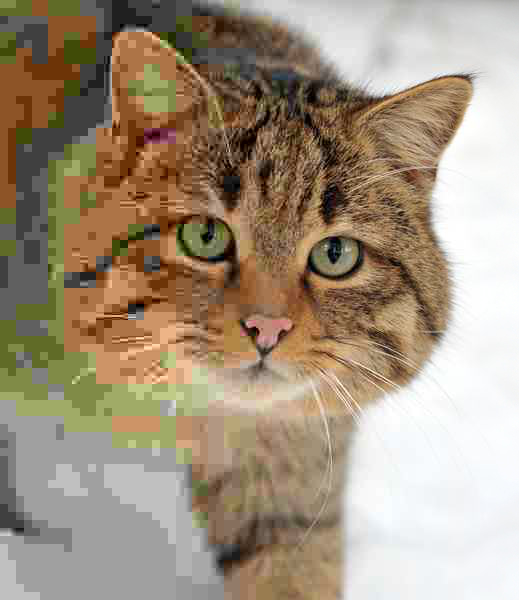
\includegraphics[width=0.40\textwidth]{fig/3-1.png}
    \captionsource{A photo of a European wildcat with the compression rate decreasing and hence quality increasing, from left to right.}
    {\url{https://en.wikipedia.org/wiki/JPEG}}
    \label{fig:jpegCompression}
\end{figure}

\vspace{2em}

\section{Algorithm}



\begin{figure}[!ht]
    \centering
    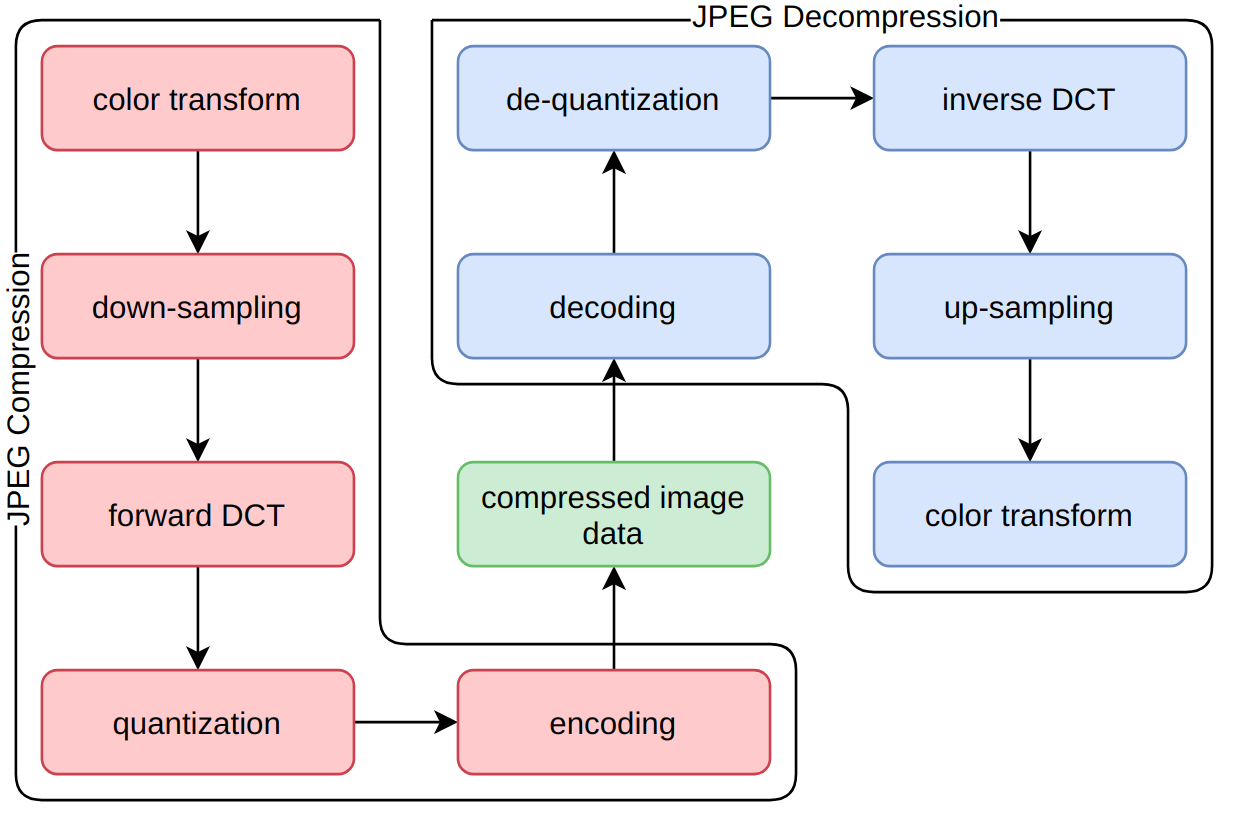
\includegraphics[width=0.80\textwidth]{fig/3-2.png}
    \caption{JPEG Schematic}
    \label{fig:jpegSchematic}
\end{figure}


\section{Conclusion}
In this chapter, we proposed a distributed algorithm
for construction of xyz.
The complexity of this algorithm is $O(n \log n)$.
Next chapter presents
another distributed algorithm which has linear time 
complexity based on xyz.

